\subsection{Reinforcement learning}

We present a Reinforcement learning (RL) based framework to explore and optimize the mapping of instructions for a given computation graph to the SE, guided by a reward function that informs the mapping algorithm about the quality of the produced mappings at each step. In this section, we give an overview of the methods used along with the formulation required for detailed description of the various components of the RL approach.

\subsection{Overview}
Proximal Policy Optimization (PPO) \cite{schulman2017proximal} is an RL method that is  widely used for continuous and discrete action problems. 
It trains an actor and a critic model (represented as neural networks).
The actor model is trained to produce actions (node placements in our case) from sample states obtained during simulation and the critic model is trained to match the sampled rewards from the actions produced by the actor using a surrogate loss function. 
This sample and train process is repeated over various iterations. 
In this manner, the problem search space is explored using the reward function as a heuristic.
Our SE mapping task is formulated as a discrete action problem where the goal is to place one node at each time step. 
Samples of SE state, actions performed and rewards obtained at each time step are collected after executing the actions provided by the actor model in simulation. 
These samples are stored in a buffer and are used as data to train the models.
Figure \ref{fig:ppo} shows the overall RL framework. 

The key components of our RL method are as follows:
\begin{itemize}
  \item States: The state is represented by a concatenation of an array of features of placed nodes, a selected node to be placed next and an embedding of the whole computation graph. 
  \item Action: The action consists of the node to be placed along with the tile and spoke location it is to be placed at.
  \item Reward function: The reward obtained is based on the number of clock cycles taken for a node to finish executing after its predecessors finished executing.
  \item Transition function: The transition function gives the probability distribution over next states given the current state and the action to be performed.
\end{itemize}

\begin{figure}[h]
  \centering
  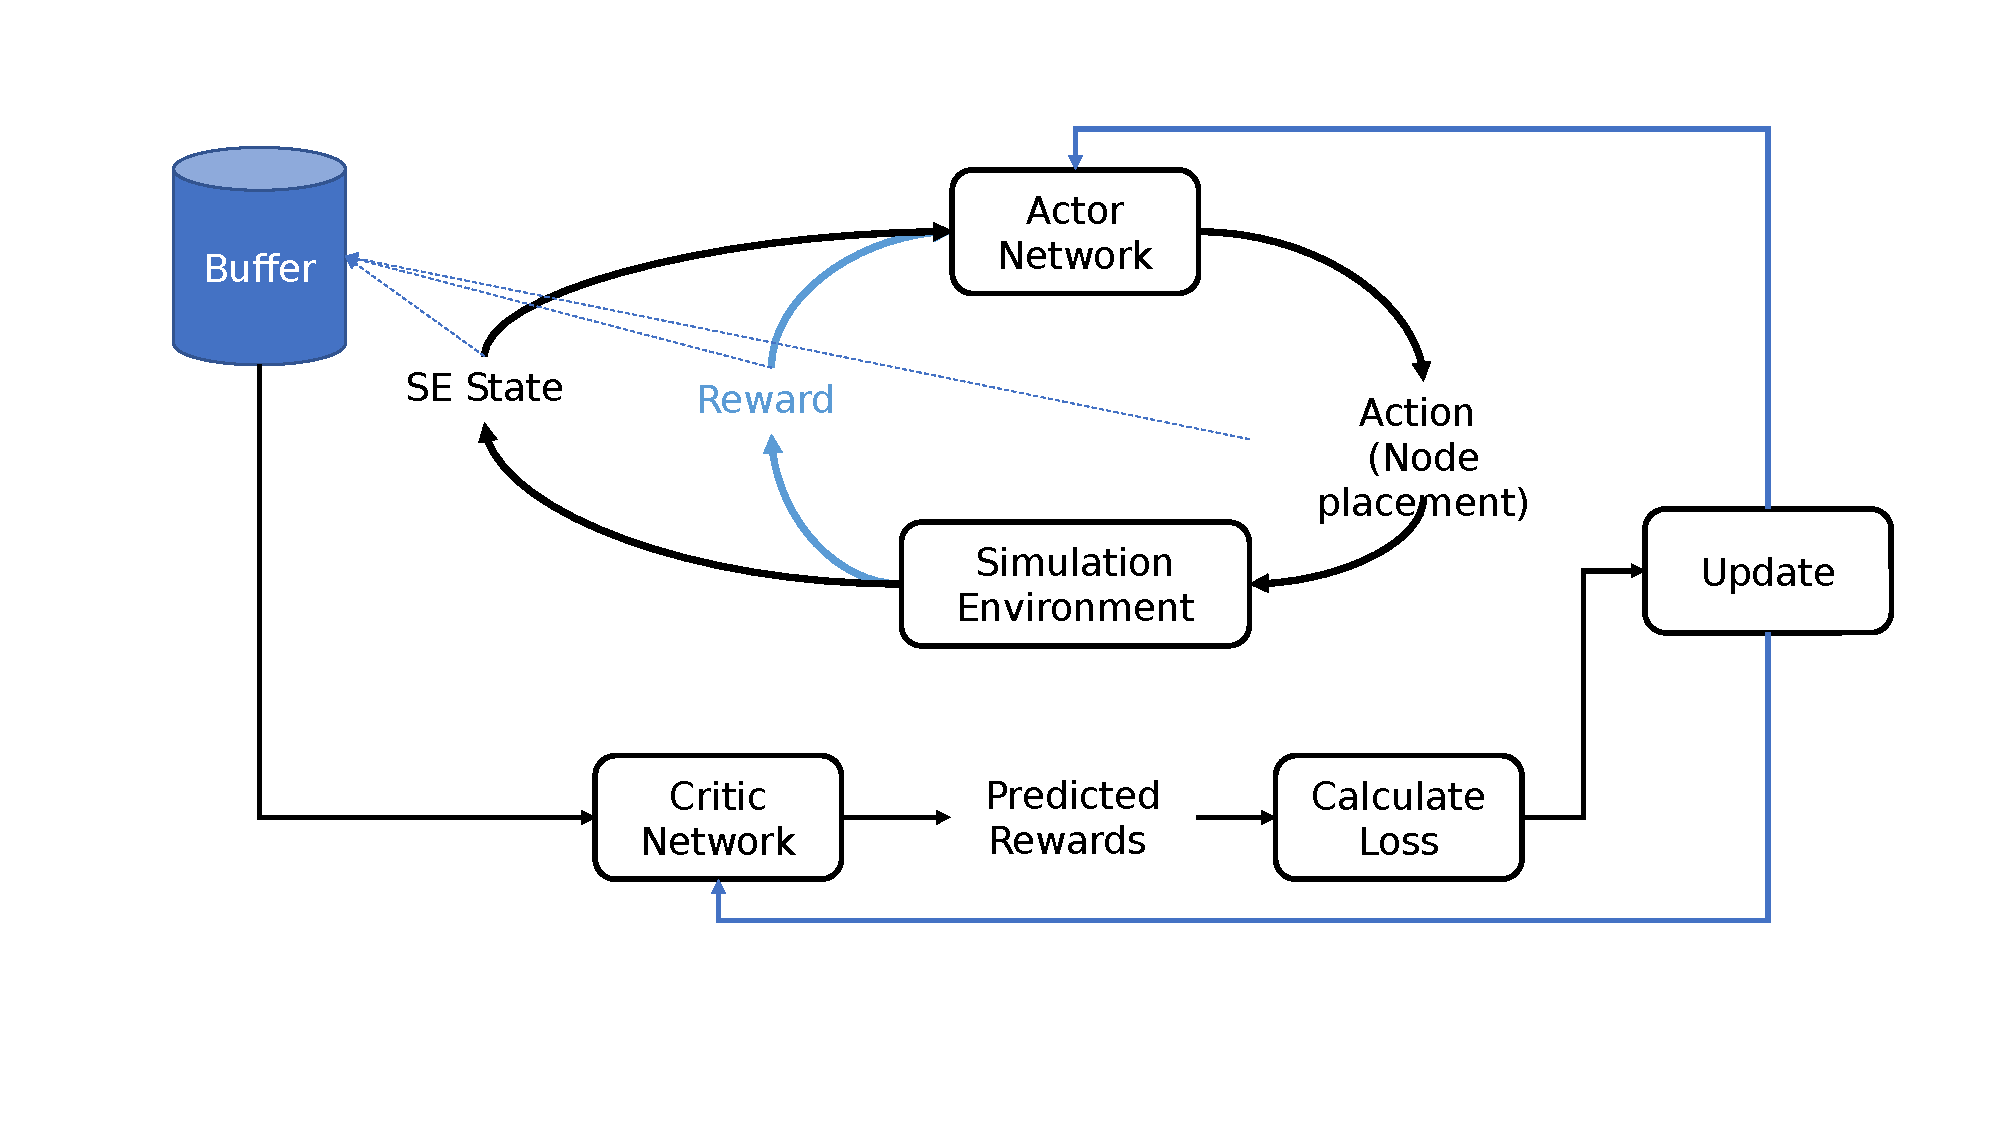
\includegraphics[width=\linewidth]{fig/ppo.pdf}
  \caption{Diagram of the RL framework showing the role of actor and critic networks during RL training. }
  \label{fig:ppo}
\end{figure}

\subsection{State Representation}
The state is a vector of size $|TS|+1$ where $TS$ is the set of tile slices in the Streaming Engine with $TS=T \times I$. Here $T$ and $I$ are sets of all tiles and initiation intervals in the SE respectively.

\subsection{Action Representation}
\todo[inline]{Ensure mathematical notations are consistent throughout paper}
The action at each step is a tuple \((n,t,i)\) where $n \in N$ (the set of all nodes) is the node to be placed and $t \in T$ and $i \in I$ are the tile and initiation interval at which the node $n$ is to be placed. 
We place nodes in a topological order which ensures that all of a node's predecessors have been placed before the node. 
We do not make selecting the node to be placed a part of the learning problem since it increases the complexity of the learning process and makes training harder.

\subsubsection{Masked Actions}
In order to enure that the network only outputs valid actions, we determine a binary mask over all possible actions and set the value of logits corresponding to invalid actions to $-\infty$ in the actor network. 
This in turn sets the probability of sampling invalid actions to $0$, ensuring that we never take an invalid action.
Finally, we only calculate entropy on valid actions, so that our algorithm maximizes exploration only on valid actions.

\subsection{Reward Function}
Our goal in this work is to get mappings that are optimal in terms of total clock cycles taken and for this purpose, the reward that is given at each time step is the difference between the clock cycle at which the current node to be placed is ready (its ready time) and the ready time of its predecessor. 
$R_n$ is the reward obtained for placing node $n$ and $t_n$ is its ready time. 
The function $p(n)$ gives the predecessor of $n$ in a computation graph. 
If the current node can't be placed because of the constraints (all values in the mask vector $m$ are zero), then a high negative reward $-\lambda$ is given.
\[
  R_n =
  \begin{cases}
    -\lambda,& m_i = 0, \, \forall \, i \in T \times I \\
    t_n - t_{p(n)}, & \text{otherwise}
    
  \end{cases}
\]

\subsection{Model design}

The architecture for actor and critic models is shown in Fig. \ref{fig:model}.
The input is separated in two categories: static and dynamic data. 
Static data is information that doesn't change as nodes are being placed, such as: computation graph and tile memory constraint.
Device state, node to be placed and placed node latencies are dynamic data that changes during placement.

Tile memory variables need to be placed in a tile so that operation can use that variable. 
This memory constraint is captured as memory dependency array. 
Tile memory constraints are incorporated into nodes in the computation graph. 
The computation graph has each node representing an instruction. 
The node features are tile memory dependencies. 
A Graph Neural Network (GNN) is used to process node dependencies and create an embedding for each node. 
An attention module is applied to the embedding matrix to select which dependency nodes are relevant to the current node to be placed. The dynamic data is fed into a MLP model to 
create another embedding to represent current state. 
The two embeddings are combined and fed into another MLP model to 
create actions. 
Invalid actions are masked before being sent to the reward function. Masking was shown to be effective in RL setting \cite{Shengyi_mask}.

\subsubsection{Global Graph Attention Module}

\begin{figure*}[h]
  \centering
  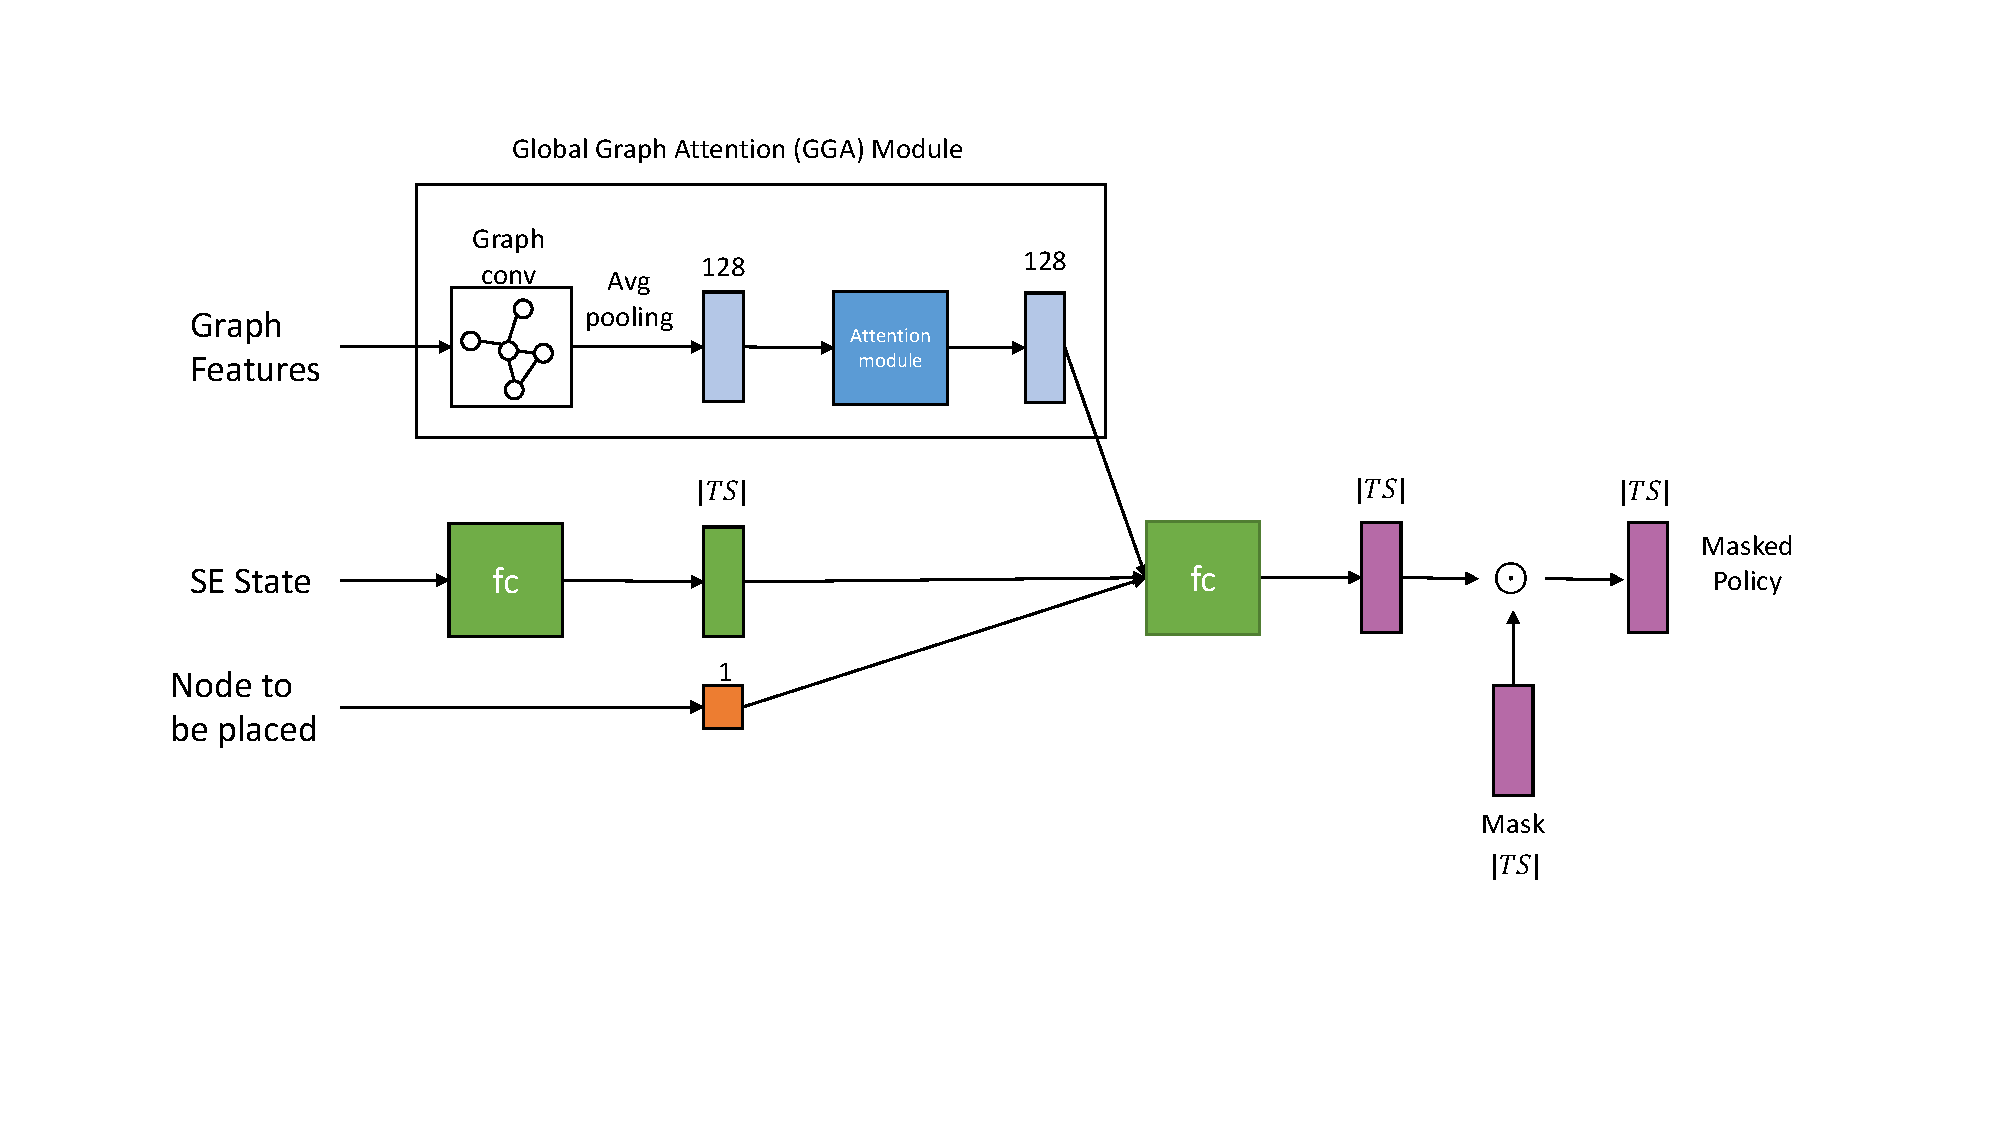
\includegraphics[width=\textwidth]{fig/model_diagram.pdf}
  \caption{Actor and critic model architecture. GNN is used to process the computation graph (static data). 
  Attention module gives importance to relevant nodes. The embedding created from dynamic data is combined with static data embedding. 
  A final MLP model is used to generate actions. Actions are masked to ensure only valid actions are produced. }
  \label{fig:model}
\end{figure*}

% \begin{algorithm*}
%   \caption{\textcolor{red}{RL Mapping Algorithm}}
%   \label{alg:mapping}
%   \begin{algorithmic}[1]
%     \State Input: $\theta_0$: Initial actor network parameters, $\phi_0$: Initial value network parameters, Graph $\mathcal{G}$ which is to be placed
%     \For{k=0,1,2,...}
%       \State Collect set of placements $\mathcal{D}_k$ by running policy $\pi(\theta_k)$.
%       \State Compute advantage estimates $\mathit{A}$ using value function $\mathit{V}$
%       \State Update policy $\pi(\theta_k)$:
%       $\theta_{k+1} = \arg \max_{\theta} \underset{s,a \sim \pi_{\theta_k}}{{\mathrm E}}\left[
%         \min\left(
%           \frac{\pi_{\theta}(a|s)}{\pi_{\theta_k}(a|s)}  A^{\pi_{\theta_k}}(s,a), \;\;
%           \text{clip}\left(\frac{\pi_{\theta}(a|s)}{\pi_{\theta_k}(a|s)}, 1 - \epsilon, 1+\epsilon \right) A^{\pi_{\theta_k}}(s,a)
%           \right)\right],$

%     \EndFor
%   \end{algorithmic}
% \end{algorithm*}

\begin{algorithm*}
  \caption{\textcolor{red}{WIP: RL Mapper Training Algorithm}}
  \label{alg1}
\begin{algorithmic}[1]
  \STATE Input: $\theta_0$: Initial actor network parameters, $\phi_0$: Initial value network parameters, Graph $\mathcal{G}$ which is to be placed
  \FOR{$k = 0,1,2,...$} 
  \STATE Collect set of node placements ${\mathcal D}_k$ by running policy $\pi(\theta_k)$.
  \STATE Compute discounted rewards $\hat{R}_t$.
  \STATE Compute advantage estimates, $\hat{A}_t = \hat{R}_t - \hat{V}_t$ using current value function $V_{\phi_k}$.
  \STATE Update the policy by maximizing the PPO-Clip objective:
      \begin{equation*}
        \theta_{k+1} = \arg \max_{\theta} \frac{1}{|{\mathcal D}_k| T} \sum_{\tau \in {\mathcal D}_k} \sum_{t=0}^T \min\left(
            \frac{\pi_{\theta}(a_t|s_t)}{\pi_{\theta_k}(a_t|s_t)}  A^{\pi_{\theta_k}}(s_t,a_t), \;\;
            g(\epsilon, A^{\pi_{\theta_k}}(s_t,a_t))
        \right),
      \end{equation*}
      via stochastic gradient ascent with Adam where
      \begin{equation}
        g(\epsilon, A) = \left\{ 
          \begin{array}{ll}
          (1 + \epsilon) A & A \geq 0 \\
          (1 - \epsilon) A & A < 0.
          \end{array}
          \right.
      \end{equation}
  \STATE Fit value function by regression on mean-squared error:
      \begin{equation*}
      \phi_{k+1} = \arg \min_{\phi} \frac{1}{|{\mathcal D}_k| T} \sum_{\tau \in {\mathcal D}_k} \sum_{t=0}^T\left( V_{\phi} (s_t) - \hat{R}_t \right)^2,
      \end{equation*}
      via gradient descent algorithm.
  \ENDFOR
\end{algorithmic}
\end{algorithm*}
